%%%%%%%%%%%%%%%%%%%%%%%%%%%%%%%%%%%%%%%%%%%%%%%%%%%%%%%%%%%%%%%%%%%%%%%%%%%%%%
% Flujoemtrias y cfd
%%%%%%%%%%%%%%%%%%%%%%%%%%%%%%%%%%%%%%%%%%%%%%%%%%%%%%%%%%%%%%%%%%%%%%%%%%%%%%
\section{Flujometrías y CFD}
%
Para obtener una mejor caracterización del funcionamiento de los puertos de
admisión y escape es necesario tener mayor conocimiento del coeficiente de
descarga para diferentes condiciones operativas de los mismos.
%
Esto se logró realizando una serie de flujometrías para obtener valores de
$C_{D}$ que sean función de la diferencia de presión que \emph{ve} el puerto y
la apertura del mismo\footnote{ICESym utiliza alzada, por lo que se traduce
área de pasaje de puerto en alzada de válvula equivalente.}, de modo obtener
$C_{D} = f(\Delta P,l_v)$.
%
El simulador ICESym requiere de información sobre el coeficiente de descarga
($C_{D}$) para calcular el área efectiva de pasaje de flujo de las válvulas o
puertos en el caso del MRCVC, introduciendo el mapa de coeficientes se tiene
una mejor aproximación al funcionamiento del sistema de intercambio de gases
porque se tiene un modelado de la eficiencia del sistema para distintos
regímenes del motor.

Las flujometrías se realizaron con \emph{OpenFOAM}, un software de de
Fluidodinámica Computacional, o CFD por sus siglas en inglés, de código libre y
abierto escrito en ``C++''.
%
% El código del programa es accesible por los usuarios, esta es una característica
% entender cómo funcionan y qué parámetros requieren algunas de las condiciones
% de contorno y post-procesadores utilizados en este trabajo.

Para realizar las simulaciones se utilizaron los \emph{solvers}
\emph{pimpleFoam} para flujo incompresible y \emph{rhoPimpleFoam} para flujo
compresible.
%
Para la turbulencia se utilizó un modelo de dos ecuaciones
\emph{$\kappa-\epsilon$}\parencite{wilcox}, este es uno de los más utilizados
y, por ser de dos ecuaciones es un modelo completo es decir, provee una
ecuación para $\kappa$ y otra para la escala de longitud turbulenta $l_m$.
%
% Este modelo requiere que se aproximen los valores iniciales de $\kappa$ y
% $\epsilon$, que a su vez requieren de la estimación de la longitud de mezcla o
% escala de la viscosidad $l_m$.

\subsection{Modelos de turbulencia}
% pag 99 (83)

El flujo a través del puerto es de carácter transitorio, turbulento.
%
Para modelar los efectos de la turbulencia se utiliza el modelo de dos
ecuaciones \emph{$\kappa-\epsilon$}, el cual brinda una ecuación para la
\emph{energía cinética turbulenta} $\kappa$ y otra para la \emph{velocidad de
disipación de la energía cinética turbulenta} $\epsilon$.
%
% El punto de partida de este (y otros) modelos de dos ecuaciones es la
% aproximación de Boussinesq

Este es uno de los modelos de dos ecuaciones más populares,

Al igual que otros modelos de dos ecuaciones, se deben definir coeficientes de
cierre y valores inicales, que se calculan a partir de:

\begin{align}
    %
  C_{\mu} &= 0.09 \\
    %
  I &= 0.05 \\
    %
  l_{m} &= 0.07 \cdot D_{m} \\
  %
  \kappa &= 1.5 \cdot {\left( u_{ref} \cdot I \right)}^{2}\\
    %
  \epsilon &= \frac{{C_{\mu}}^{3/4} \cdot {\kappa}^{3/2}} {l_{m}}
    %
\end{align}

Dónde:
%
\begin{itemize}

    \item $C_{\mu}$, es un coeficiente propio del modelo.
        %
    \item I, es la intensidad de turbulencia estimada, en este trabajo se utilizó 0.05.
        %
    \item $l_m$, es la longitud de mezcla o escala de viscosidad,
     para flujos internos se suele usar el diámetro hidráulico de la cañería.
        %
    \item $\kappa$, es la energía cinética turbulenta.
        %
    \item $\epsilon$, es la disipación de energía cinética turbulenta.
        %
\end{itemize}

% https://www.openfoam.com/documentation/guides/latest/doc/guide-turbulence-ras-k-epsilon.html
La longitud de mezcla $l_m$ determina el tamaño que pueden tener los \emph{eddys}
turbulentos, su valor inicial se aproximó como la altura de cámara $l_m = h_c$.


\subsection{Condiciones Iniciales}
%
Las condiciones iniciales se determinan para cada punto de interés a partir de
los datos obtenidos del simulador ICESym.
%
Las variables básicas que se utilizan para calcular los parámetros propios del
modelo son presión, temperatura, densidad y velocidad; a partir de estos se
calculan el resto de los valores necesarios.
%

El modelo $\kappa-\epsilon$ estándar es:

% eddy viscosity
\begin{equation}
  \mu_{T}=\rho C_{\mu}k^{2}/\epsilon
\end{equation}

% Turbulence Kinetic Energy
\begin{equation}
  \rho\frac{\delta k}{\delta t}
  \rho U_{j}\frac{\delta k}{\delta x_{j}}
  =
  \tau_{ij} \frac{\delta U_{i}}{\delta x_{j}}
  -
  \rho\epsilon
  +
  \frac{\delta}{\delta x_{j}}\left[
    (\mu + \mu_{T}/\sigma_{k})\frac{\delta k}{\delta x_{j}}
  \right]
\end{equation}

% Dissipation Rate
\begin{equation}
  \rho\frac{\delta \epsilon}{\delta t}
  \rho U_{j}\frac{\delta \epsilon}{\delta x_{j}}
  =
  C_{\epsilon 1}\frac{\epsilon}{k} \tau_{ij}\frac{\delta U_{i}}{\delta x_{j}}
  -
  C_{\epsilon 2 \rho}
  \frac{\epsilon^{2}}{k}
  +
  \frac{\delta}{\delta x_{j}}\left[
    (\mu + \mu_{T}/\sigma_{T})\frac{\delta \epsilon}{\delta x_{j}}
  \right]
\end{equation}

% Clossure Coefficient

En la tabla~\ref{tab:condiciones_iniciales} se muestran los datos necesarios
para las flujometrías, separados en flujo incompresibles (pimpleFoam) y
compresibles (rhoPimpleFoam).

\begin{table}
\centering
    \begin{tabular}{rccc} \toprule
      Variable      & Descripción   & Incompresible & Compresible \\ \midrule
      $\epsilon$    &               &               & \\
      $\kappa$      &               &               & \\
      $\gamma$      &               &               & \\
      $\mu$         &               &               & \\
      $\nu$         &               &               & \\
      $M_{w}$       &               &               & \\
      $P_{r}$       &               &               & \\
      $\rho$        &               &               & \\
      $P_{puerto}$  &               &               & \\
      $P_{cámara}$  &               &               & \\
      $V_{puerto}$  &               &               & \\
      $T_{puerto}$  &               &               & \\
      $T_{cámara}$  &               &               & \\ \bottomrule
    \end{tabular}
    \caption{Condiciones Iniciales}\label{tab:condiciones_iniciales}
\end{table}

No se considera la transferencia de calor en las paredes.

Debido a la cantidad de flujometrías a realizar, se utilizó un script para leer
los datos de salida de ICESym y calcular los valores requeridos en función del
tipo de simulador a utilizar.

%%%%%%%%%%%%%%%%%%%%%%%%%%%%%%%%%%%%%%%%%%%%%%%%%%%%%%%%%%%%%%%%%%%%%%%%%%%%%%%

\subsection{Metodología}
%
El esquema de trabajo para realizar las simulaciones consistió en:

\begin{enumerate}
        %
    \item Pre-procesado
      %
        \begin{enumerate}
                %
            \item Definir la geometría a analizar.
              %
            \item Generar una malla con un tamaño de elemento adecuado, la
                solución a problemas de CFD depende fuertemente de la cantidad
                y tamaño de celdas utilizadas.
              %
            \item Seleccionar los modelos adecuados.
              %
            \item Definir las propiedades del fluido.
              %
            \item Definir las condiciones de borde.

              %
        \end{enumerate}
        %
    \item Solver
      %
    \begin{enumerate} \item Seleccionar el solver a utilizar.
            %
            \item Ejecutar la simulación.
            %
    \end{enumerate}
        %
\item Post-procesado
      %
    \begin{enumerate}
                %
        \item Visualizar los resultados de las distintas variables de la
            simulación.
            %
        \item Extraer la información necesaria.
            %
    \end{enumerate}
        %
\end{enumerate}

%%%%%%%%%%%%%%%%%%%%%%%%%%%%%%%%%%%%%%%%%%%%%%%%%%%%%%%%%%%%%%%%%%%%%%%%%%%%%%%

\subsubsection{Pre procesado}
%
El preprocesado consiste en definir geometría y condiciones iniciales, esto se
obtiene de las simulaciones con ICESym, en la que se identificaron los puntos
de interés luego de representar la diferencia de presión en función de la
alzada para todo el régimen de operación del motor, (1000 a 9000 RPM).
% Se definió el dominio de la simulación a partir de la geometría obtenida de
% la optimización con el algoritmo genético del motor utilizando coeficientes
% de descarga constantes para el flujo a través de los puertos.
%
%
La geometría para las posiciones de interés se volcó en un modelo de CAD
paramétrico que se obtuvo realizando sumas, restas, uniones e intersecciones de
volúmenes que representan diferentes componentes del motor.
%
En la figura~\ref{fig:admision_50} se muestra parte del proceso para obtener el
puerto de admisión a $\theta=50^{\circ}$, en donde se suma el volumen del mismo
en gris y las figuras que se restan que corresponden al rotor, las paletas y un
paralelogramo para quitar una región que no se simuló.

\begin{figure}
    \centering
    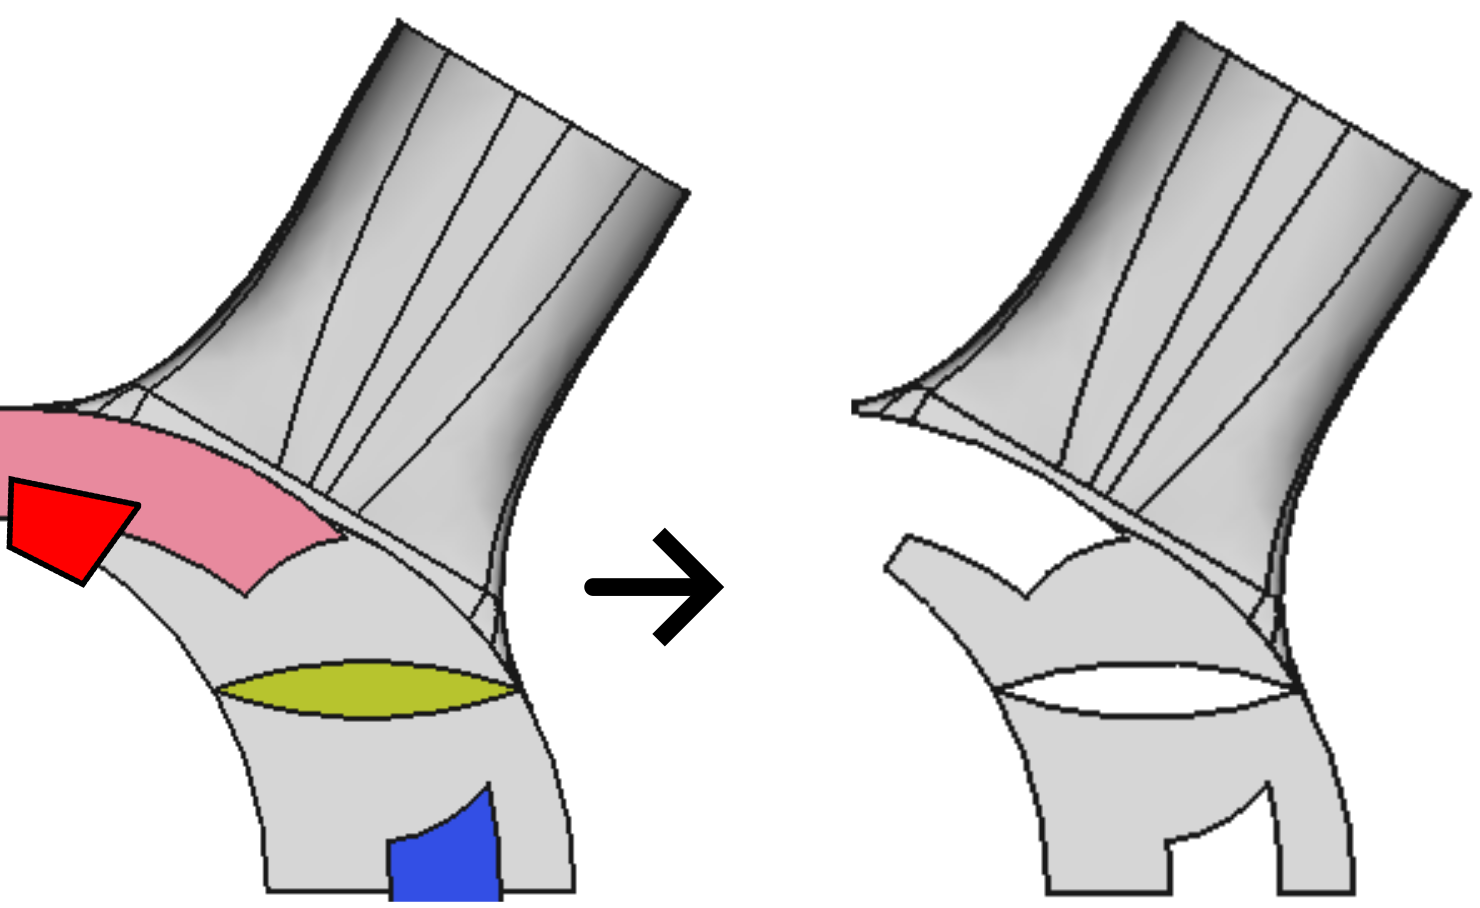
\includegraphics[width=0.7\textwidth]{./CAD/freecad_pasos.png}
    \caption{FreeCAD, Operaciones Booleanas}\label{fig:admision_50}
\end{figure}

Esta geometría fue generada por el programa FreeCAD~\parencite{freecad},
exportada a un archivo
``.BREP''\footnote{\href{https://dev.opencascade.org/doc/overview/html/specification\_\_brep\_format.html}{Formato
BREP, opencascade.org}} para luego ser importada en Salome\parencite{salome},
%
Este programa se utilizó para generar una malla cerrada o  \emph{weatertight}
necesaria para ser procesada por los complementos de OpenFOAM utilizados para
generar la malla que se vuelve el dominio de la simulación, \emph{blockMesh} y
\emph{snappyHexMesh}.
%
Es importante que la malla sea de hermética y que los nodos en la frontera
entre superficies coincidan, como se ve en la figura
\ref{fig:salome_malla_hermetica}, en la que se ven dos superficies "walls" y
"outlet".
%
Esto es necesario porque snappyHexMesh parte de una malla como la generada por
blockMesh y la intersección de la misma con la superficie de un archivo (en
este caso) ".stl".
%
Se debe indicar un punto dentro o fuera de esta superficie \emph{stl},
dependiendo del lado/cara por la que va a simularse el flujo, esto dependerá si
se va a simular un flujo externo o interno.
%
En el caso de estudio todos los flujos son internos por lo que se define una
caja que encierra la totalidad del volumen de la malla \emph{stl} creada por
salome.

\begin{figure}
    \centering
    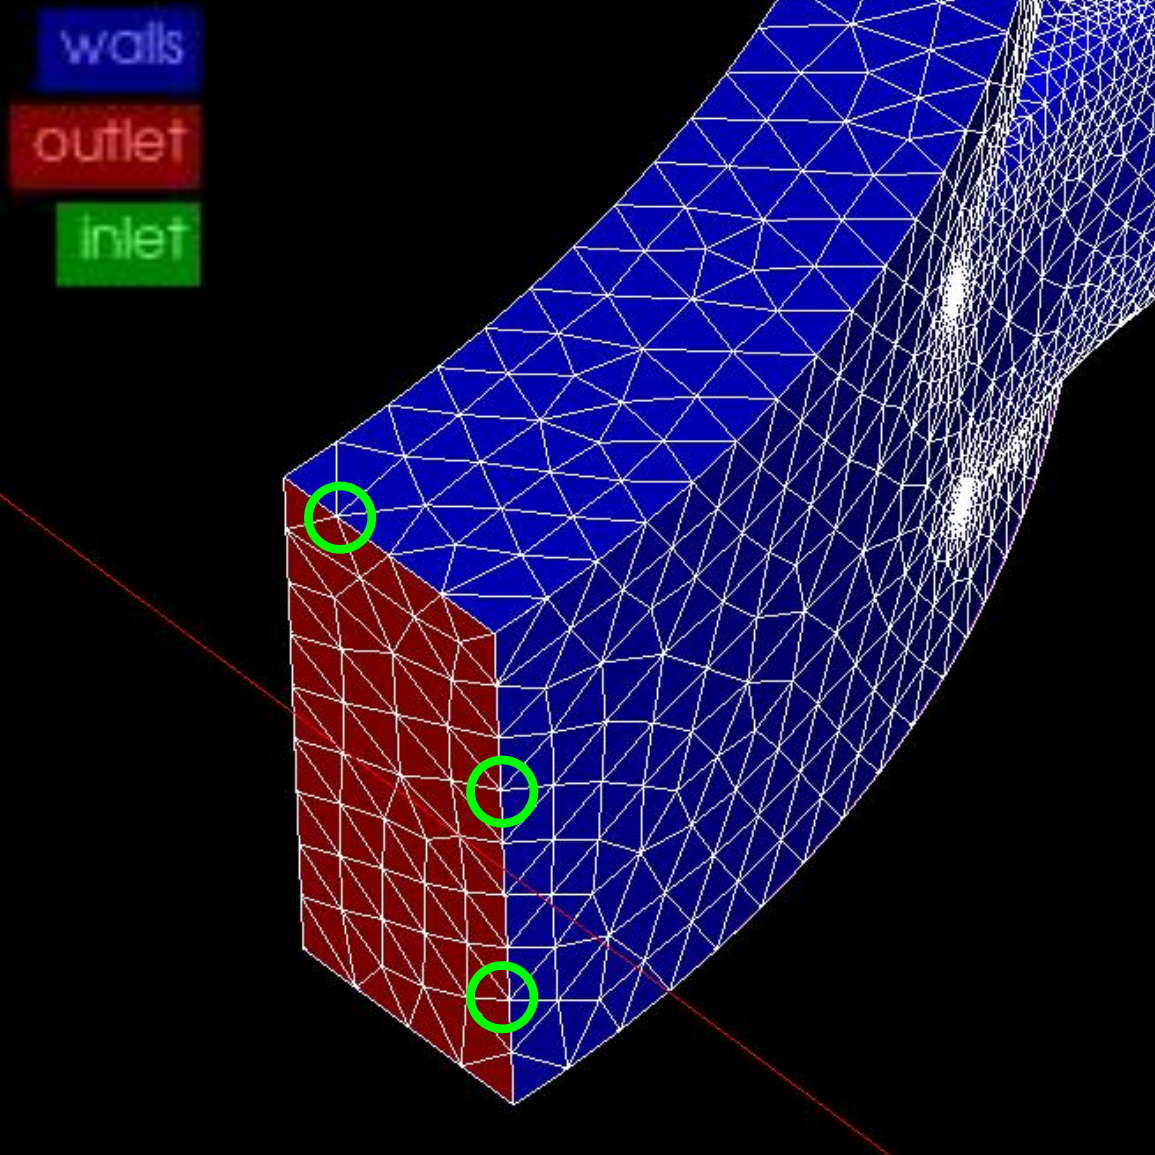
\includegraphics[width=0.5\textwidth]{./flujometrias/salome_malla_hermetica.png}
    \caption{Malla hermética}\label{fig:salome_malla_hermetica}
\end{figure}

El proceso en Salome consta de importar la geometría generada por FreeCAD y
separar la misma en superficies, a las cuales se le da un nombre que se
utilizará para definir dicha cara o parche.
%
Estos nombres son necesarios para definir condiciones de contorno en OpenFOAM.

Luego de separadas las caras en paredes, entradas y salidas, se procede a
generar la malla en formato stl con el complemento Malla del software.
%
Se utilizó el generador de mallas NETGEN 1D-2D para crear la superficie stl, en
general se configuró el mallador de modo de tener un stl de buena calidad con
elementos de menor tamaño en zonas de mayor curvatura.
%
En la figura \ref{fig:salome_fina_gruesa} se ve la diferencia en cantidad de
nodos de dos mallas, una malla fina a la izquierda y una malla gruesa a la
derecha las configuración de cada malla se muestra en la tabla \ref{tab:salome_fina_gruesa}.
%
Esto sin requerir de una gran cantidad de elementos para no ralentizar el
procesado con snappyHexMesh,

\begin{figure}[t!]
    \centering
    \begin{subfigure}[t]{0.5\textwidth}
        \centering
        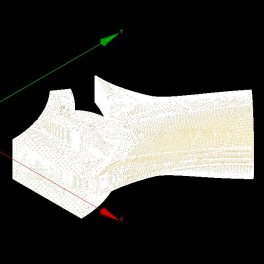
\includegraphics{./flujometrias/salome3_fina.png}
        \caption{Malla fina sin optimizar}
    \end{subfigure}%
    \begin{subfigure}[t]{0.5\textwidth}
        \centering
        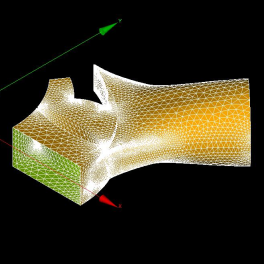
\includegraphics{./flujometrias/salome3_gruesa.png}
        \caption{Malla gruesa optimizada}
    \end{subfigure}
    \caption{Diferentes mallas para flujometrías}\label{fig:salome_fina_gruesa}
\end{figure}

\begin{table}
    \centering
    \begin{tabular}{lcc} \toprule
        Parámetro                & Malla Fina    & Malla Gruesa \\ \midrule
        Tamaño máximo            & 0.001         & 0.03 \\
        Tamaño mínimo            & 1E-7          & 2.4E-5 \\
        Limitado por curvatura   & Sí            & Sí \\
        Optimizar                & No            & Sí \\
        Cantidad de nodos        & 99311         & 49112 \\
        Cantidad de elementos    & 204695        & 103163 \\ \bottomrule
    \end{tabular}
    \caption{Configuración de mallas mostradas en la figura \ref{fig:salome_fina_gruesa}}
    \label{tab:salome_fina_gruesa}
\end{table}

Una vez obtenido el archivo STL con la calidad deseada, se procede a la
generación de la malla dentro de OpenFOAM con blockMesh y snappyHexMesh.


%%%%%%%%%%%%%%%%%%%%%%%%%%%%%%%%%%%%%%%%%%%%%%%%%%%%%%%%%%%%%%%%%%%%%%%%%%%%%%%

\subsubsection{Geometría}
%
Previo a definir otros detalles de las flujometrías, es necesario definir
alguna nomenclatura para la geometría, nombre asignado a superficies como
paredes, entrada, salida y cámara de combustión.
%
El resto de las superficies se definen como paredes \emph{wall}.


%%%%%%%%%%%%%%%%%%%%%%%%%%%%%%%%%%%%%%%%%%%%%%%%%%%%%%%%%%%%%%%%%%%%%%%%%%%%%%%
% NOTA: para esta sección, meter algo como lo que está aca abajo:
% Para las flujometrías en las que no hay solape de cámaras, se definen las
% propiedades de una entrada y una cámara de combustión, indicadas como
% \emph{port} y \emph{chamber} respectivamente como se ve en la
% figura~\ref{fig:ref_geom1}.
% %
% (Figura aca)

El puerto y la cámara de combustión (o cámaras en caso de que haya solape), se
definen como \emph{patch}, una frontera permeable.

%%%%%%%%%%%%%%%%%%%%%%%%%%%%%%%%%%%%%%%%%%%%%%%%%%%%%%%%%%%%%%%%%%%%%%%%%%%%%%%
\subsection{Coeficiente de descarga ($C_D$)}

El coeficiente másico se calcula a partir de las ecuaciones de flujo
compresible a través de una restricción, para el caso en que el flujo no esté
bloqueado, la ecuación de $\dot{m}$ es:

\begin{equation}
    \label{eq:m_not_choked}
    \dot{m} = \frac{C_D A_R p_0}{\sqrt{R T_0}}
            {\left(\frac{p_T}{p_0} \right)}^{1/\gamma}
            {\left( \frac{2\gamma}{\gamma-1} \left[1- {(\frac{p_T}{p_0})}^{{\gamma-1}/\gamma} \right] \right)}^{1/2}
\end{equation}

En caso del que el flujo esté bloqueado, es decir
$p_T/p_0 \le {[2/\gamma+1]}^{\gamma/(\gamma - 1)}$
, la ecuación correspondiente es:

\begin{equation}
  \dot{m}=  \frac {C_D A_R p_0} {{(R T_0)}^{1/2}}
            \gamma^{1/2}
            {\left( \frac{2\gamma}{\gamma+1} \right)}^{(\gamma+1)/(2(\gamma-1))}
\end{equation}

Para determinar $C_D$ se debe conocer:

\begin{itemize}
    \item $p_0$, es la presión de estancamiento antes de la restricción.
    \item $T_0$, es la temperatura de estancamiento antes de la restricción.
    \item $p_T$, es la presión estática justo después de la restricción.
    \item $A_R$, es el área de referencia.
    \item $\dot{m}$, es el caudal másico.
    \item $\gamma$, es el cociente de capacidades térmicas del gas.
\end{itemize}

El área de referencia utilizada en ICESym es el área frontal del puerto expuesta
a la cámara que se esté analizando, calculada como $A_{R} = h_{p} \cdot l_{{v}}$.
%
Debido a que el MRCVC no tiene válvulas, en trabajos anteriores se confeccionó
un script para calcular la distancia $l_v$ en función del ángulo del ciclo.
%
En la figura~\ref{fig:area_referencia} se ilustran las áreas de referencia para
una posición del rotor en la que hay solape de cámaras con $\theta = 55^\circ$.

\begin{figure}
    \centering
    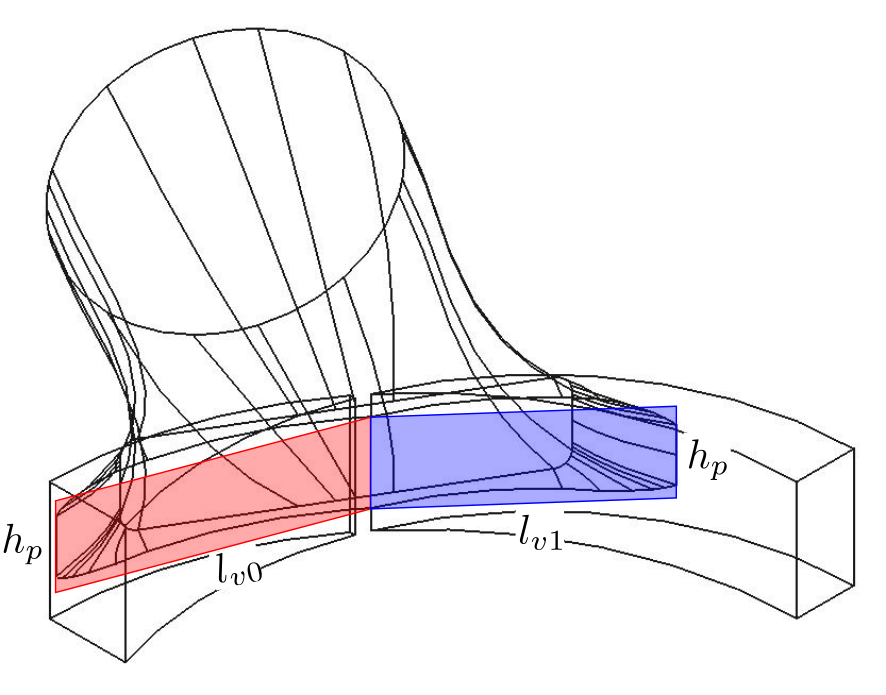
\includegraphics[]{area_referencia.png}
    \caption{Área de referencia}\label{fig:area_referencia}
\end{figure}

Los valores de densidad, velocidad, presión y temperatura se obtienen de los
datos de salida de ICESym para un puerto, ángulo y velocidad dada, en
particular del archivo de salida con nombre \emph{$cyl_0.txt$} que contiene
información relevante a la cámara de combustión.
%
Para la temperatura se utiliza la temperatura de cámara, $T_0 = T_C$, la
presión antes y después del puerto se selecciona de acuerdo al sentido de
flujo, en caso de ser flujo hacia la cámara de combustión, la presión en el
puerto se utiliza como inicial $P_0$ y la presión en la cámara es la
aproximación a la presión en la restricción $P_T$.

Para inicializar el campo de presión y densidades, se usa la media entre las
cámaras que se estén simulando y se establece un campo uniforme.

La velocidad se inicializa con un campo nulo de velocidades, que en la
configuración de OpenFOAM se designa como \emph{internalField uniform (0 0 0)}.

En resumen, los valores iniciales de los campos de presión, temperatura y velocidad
son los indicados en la tabla~\ref{tab:cc}.

\begin{table}
\centering
    \begin{tabular}{cccc} \toprule
        Var & Campo         & Parche                      & Pared \\
        T   & uniforme T0   & inletOutlet                 & uniforme T9\\ \midrule
        P   & uniform Pavg  & uniformTotalPressure        & Pi \\
        U   & uniform (0 0 0) & pressureInletOutletVelocity & valor fijo (0 0 0)\\
        rho & uniform rhoAvg \\ \bottomrule
    \end{tabular}
    \caption{Condiciones de Borde}\label{tab:cc}
\end{table}

En todos los casos se tomará como velocidad de referencia a la media entre la
velocidad en la punta del tubo de las cámaras solapadas.
%
Del mismo modo, la temperatura será la temperatura de cámara media.

Si hay o no solape de cámaras va a depender tanto de la geometría del puerto
como de la posición del ciclo en la que se encuentre, para determinar las
condiciones iniciales se debe tener en cuenta el solape.
%
En la figura~\ref{fig:geom} se muestra un corte del puerto con un plano cuya
normal está en $\vec{z}$, se denominará a la cámara que esté a la izquierda
como cámara 0 y a la que esté a la derecha cámara 1
%
Al haber solape de cámaras, para definir la presión del puerto y estimar las
condiciones iniciales de los parámetros viscosos que requiere el modelo
$k-\epsilon$ se utilizan valores medios de presión, velocidad y temperatura de
ambas cámaras.
%
Además, las condiciones iniciales de que se aplican al parche denominado
\emph{puerto} es igual a la media aritmética de la velocidad de las velocidades
de los puertos de ambas cámaras, Lo mismo sucede con la presión, densidad y
temperatura.

A partir de estos datos se calculan varias propiedades termodinámicas del gas,
incluyendo la constante del gas, masa molar, viscosidad cinemática y demás.
%
Para calcular estas propiedades se asume que el gas no contiene gases
residuales.

Finalmente el caudal másico yse obtiene con OpenFOAM, en donde se simula el
tiempo suficiente para que los caudales másicos por entradas o salidas se
estabilice, como se ve en la figura~\ref{fig:caudalMasico}.

\begin{figure}
    \centering
    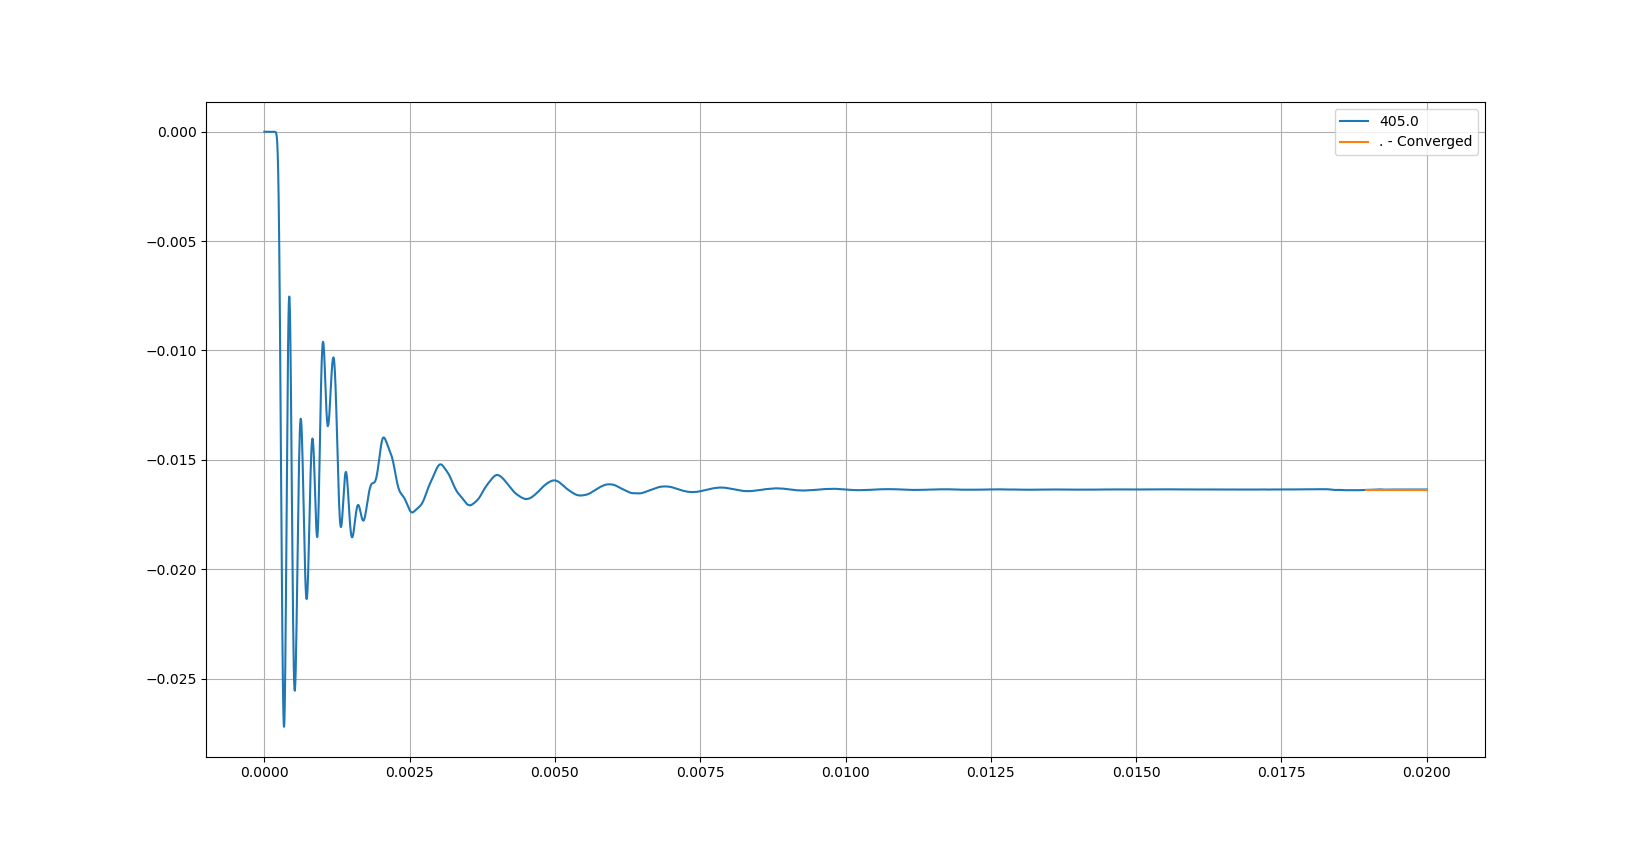
\includegraphics[width=0.6\textwidth]{surfaceFieldValue_405.0.png}
    \caption{Flujometrías para el puerto de Admisión}\label{fig:caudalMasico}
\end{figure}
En todos los casos se tomará como velocidad de referencia a la media entre la
velocidad en la punta del tubo de las cámaras que se estén solapando.
%
Del mismo modo, la temperatura será la temperatura de cámara media.

Si hay o no solape de cámaras va a depender tanto de la geometría del puerto
como de la posición del ciclo en la que se encuentre, para determinar las
condiciones iniciales se debe tener en cuenta el solape.
%
En la figura~\ref{fig:geom} se muestra un corte del puerto con un plano cuya
normal está en $\vec{z}$, se denominará a la cámara que esté a la izquierda
como cámara 0 y a la que esté a la derecha cámara 1
%
Al haber solape de cámaras, para definir la presión del puerto y estimar las
condiciones iniciales de los parámetros viscosos que requiere el modelo
$k-\epsilon$ se utilizan valores medios de presión, velocidad y temperatura de
ambas cámaras.
%
Además, las condiciones iniciales de que se aplican al parche denominado
\emph{puerto} es igual a la media aritmética de la velocidad de las velocidades
de los puertos de ambas cámaras, Lo mismo sucede con la presión, densidad y
temperatura.


%%%%%%%%%%%%%%%%%%%%%%%%%%%%%%%%%%%%%%%%%%%%%%%%%%%%%%%%%%%%%%%%%%%%%%%%%%%%%%%

OpenFOAM is a free, open source computational fluid dynamics (CFD) software
package released by the OpenFOAM Foundation.
%
It has a large user base across most areas of engineering and science, from both
commercial and academic organisations.
%
OpenFOAM has an extensive range of features to solve anything from complex fluid
flows involving chemical reactions, turbulence and heat transfer, to solid
dynamics and electromagnetics.
